\section{目录和路径名}
\subsection{目录}
最早的文件系统设计简单,只使用文件名来标识文件。这种方法带来了管理上的挑战,因为文件名的唯一性限制了归档和检索的灵活性。随着时间的推移,我们逐渐采用了按功能、属性分类文件的方式,将文件整理到不同层级的目录中。这种层级结构使得我们能够更轻松地逐级定位所需文件。

目录的引入不仅使得文件组织更加清晰,还改善了文件访问权限的管理。通过目录,我们可以间接地控制用户或用户组对特定目录下所有文件的访问权限。这简化了操作系统对多用户环境下文件访问的安全管理。

同时,通过使用Linux系统中的stat工具,我们可以获取目录的相关信息。这些信息包括目录的权限、所有者、大小以及创建或修改时间等。这些数据对于了解和管理文件系统的结构和属性至关重要,有助于维护和控制文件系统的安全性和可靠性。stat工具使用实例如下:

\begin{lstlisting}[language=Rust]
$ stat oskernel2022-npucore
File: oskernel2022-npucore
Size: 4096          Blocks: 8          IO Block: 4096   directory
Device: 805h/2053d    Inode: 589840      Links: 15
Access: (0775/drwxrwxr-x)  Uid:(1000/ubuntu)   Gid: (1000/ubuntu)
Access: 2023-12-14 21:24:40.479999513 +0800
Modify: 2023-12-02 23:54:03.232637849 +0800
Change: 2023-12-02 23:54:03.232637849 +0800
Birth: -
\end{lstlisting}

\textbf{File}表明它的文件名为oskernel2022-npucore。

\textbf{Size}表明它的字节大小为4096字节。

\textbf{Blocks}表明它占据 8 个块 (Block) 来存储。在文件系统中,文件的数据以块为单位进行存储。在 IO Block 可以看出,在 Linux操作系统中的Ext4文件系统的每个块的大小为 4096 字节。

\textbf{directory}表明oskernel2022-npucore是一个目录,该位置为\textbf{regular file}时表明这个文件是一个常规文件。事实上,其他类型的文件也可以通过文件名来进行访问。

当文件是一个特殊文件(如块设备文件或者字符设备文件)的时候,Device将指出该特殊文件的 major/minor ID。

\textbf{Inode}表示文件的底层编号。在文件系统的底层实现中,并不是直接通过文件名来索引文件,而是首先需要将文件名转化为文件的底层编号,再根据这个编号去索引文件。目前我们无需关心这一信息。

\textbf{Links}给出文件的硬链接数。同一个文件系统中如果两个文件(目录也是文件)具有相同的inode号码,那么就称它们是“硬链接”关系。这样links的值其实是一个文件的不同文件名的数量。

\textbf{Uid}给出该文件的所属的用户 ID ,\textbf{Gid}给出该文件所属的用户组 ID 。Access的其中一种表示是一个长度为 10 的字符串(这里是 drwxrwxr-x ),其中第 1 位给出该文件的类型,这个文件是一个目录,因此这第 1 位为d。后面的 9 位可以分为三组,分别表示该文件的所有者/在该文件所属的用户组内的其他用户以及剩下的所有用户能够读取/写入/将该文件作为一个可执行文件来执行。

\textbf{Access/Modify}分别给出该文件的最近一次访问/最近一次修改时间。

实际上目录也可以看作一种文件,它也有属于自己的底层编号,它的内容中保存着若干 \textbf{目录项} (Dirent, Directory Entry),可以看成一组映射,根据它下面的文件名或子目录名能够查到文件和子目录在文件系统中的底层编号,即 Inode 编号。但是与常规文件不同的是,用户无法
\textbf{直接}修改目录的内容,只能通过创建/删除它下面的文件或子目录才能间接做到这一点。

\subsection{路径}
有了目录之后,我们就可以将所有的文件和目录组织为一种被称为
\textbf{目录树} (Directory Tree) 的有根树结构(不考虑软链接)。树中的
每个节点都是一个文件或目录,一个目录下面的所有的文件和子目
录都是它的孩子。可以看出所有的文件都是目录树的叶子节点。目
录树的根节点也是一个目录,它被称为\textbf{ 根目录} (Root Directory)。
目录树中的每个目录和文件都可以用它的\textbf{ 绝对路径 }(Absolute
Path) 来进行索引和定位。绝对路径是目录树上的根节点到待索引
的目录和文件所在的节点之间自上而下的路径。此路径上的所有节
点(文件或目录)两两之间加上路径分隔符拼接就可得到绝对路径
名。例如,在 Linux 上,根目录的绝对路径是 “/” ,路径分隔符
也是 “/” ,因此:

一般情况下,绝对路径都很长,用起来颇为不便。而且,在日常
使用中,我们通常固定在一个工作目录下而不会频繁切换目录。因
此更为常用的是 \textbf{相对路径} (Relative Path) 而非绝对路径。每个进程都会记录自己当前所在的工作目录(Current Working
Directory, CWD),当它在索引文件或目录的时候,如果传给它的
路径并未以 / 开头,则会被内核认为是一个相对于进程当前工
作目录的相对路径。这个路径会被拼接在进程当前路径的后面组成
一个绝对路径,实际索引的是这个绝对路径对应的文件或目录。其
中, ./ 表示当前目录,而 ../ 表示当前目录的父目录,这在
通过相对路径进行索引的时候非常实用。在使用终端的时候,执行pwd 命令可以打印终端进程当前所在的目录,而通过 cd 可以
切换终端进程的工作目录。

一旦引入目录之后,我们就不再单纯的通过文件名来索引文件,而
是通过路径(绝对或相对)进行索引。在文件系统的底层实现中,
也是对应的先将路径转化为一个文件或目录的底层编号,然后再通
过这个编号具体索引文件或目录。将路径转化为底层编号的过程是
逐级进行的,对于绝对路径的情况,需要从根目录出发,每次根据
当前目录底层编号获取到它的内容,根据下一级子目录的目录名查
到该子目录的底层编号,然后从该子目录继续向下遍历,依此类
推。在这个过程目录的权限控制位将会起到保护作用,阻止无权限
用户进行访问。

\subsection{NPUCore中目录树的数据结构及具体实现}
NPUCore中具体实现方式是通过文件目录树来实现的,目录树(Directory Tree)的有根树数据结构如下所示。

\begin{figure}[H]
	\centering
	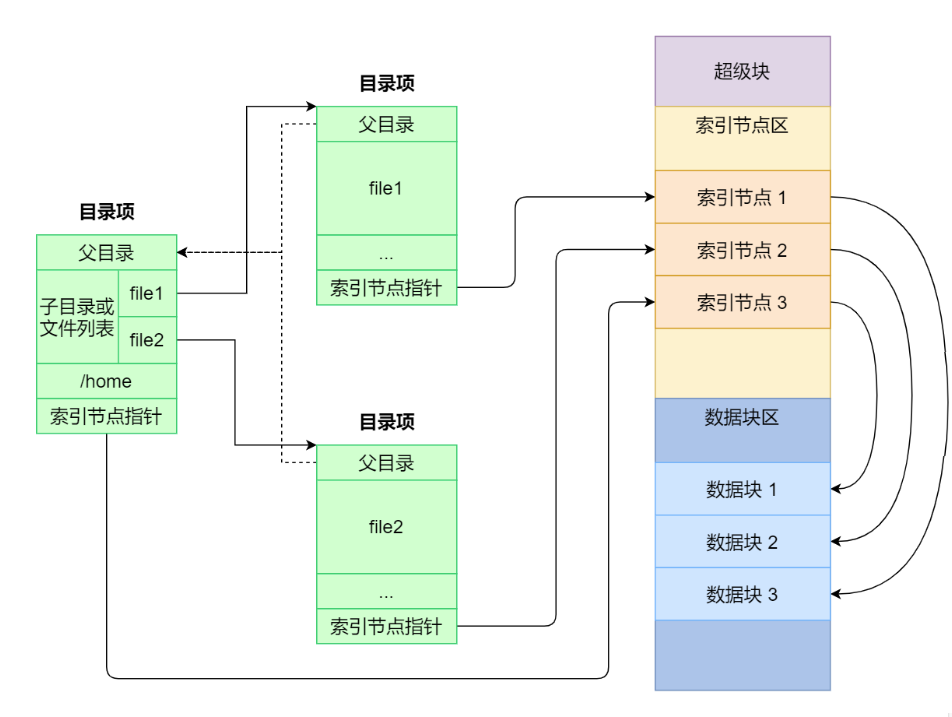
\includegraphics[width=14cm,height=11cm]{figures/07-05-目录树的有根树数据结构.png}
	\caption{目录树的有根树数据结构}
\end{figure} 

\begin{figure}[H]
	\centering
	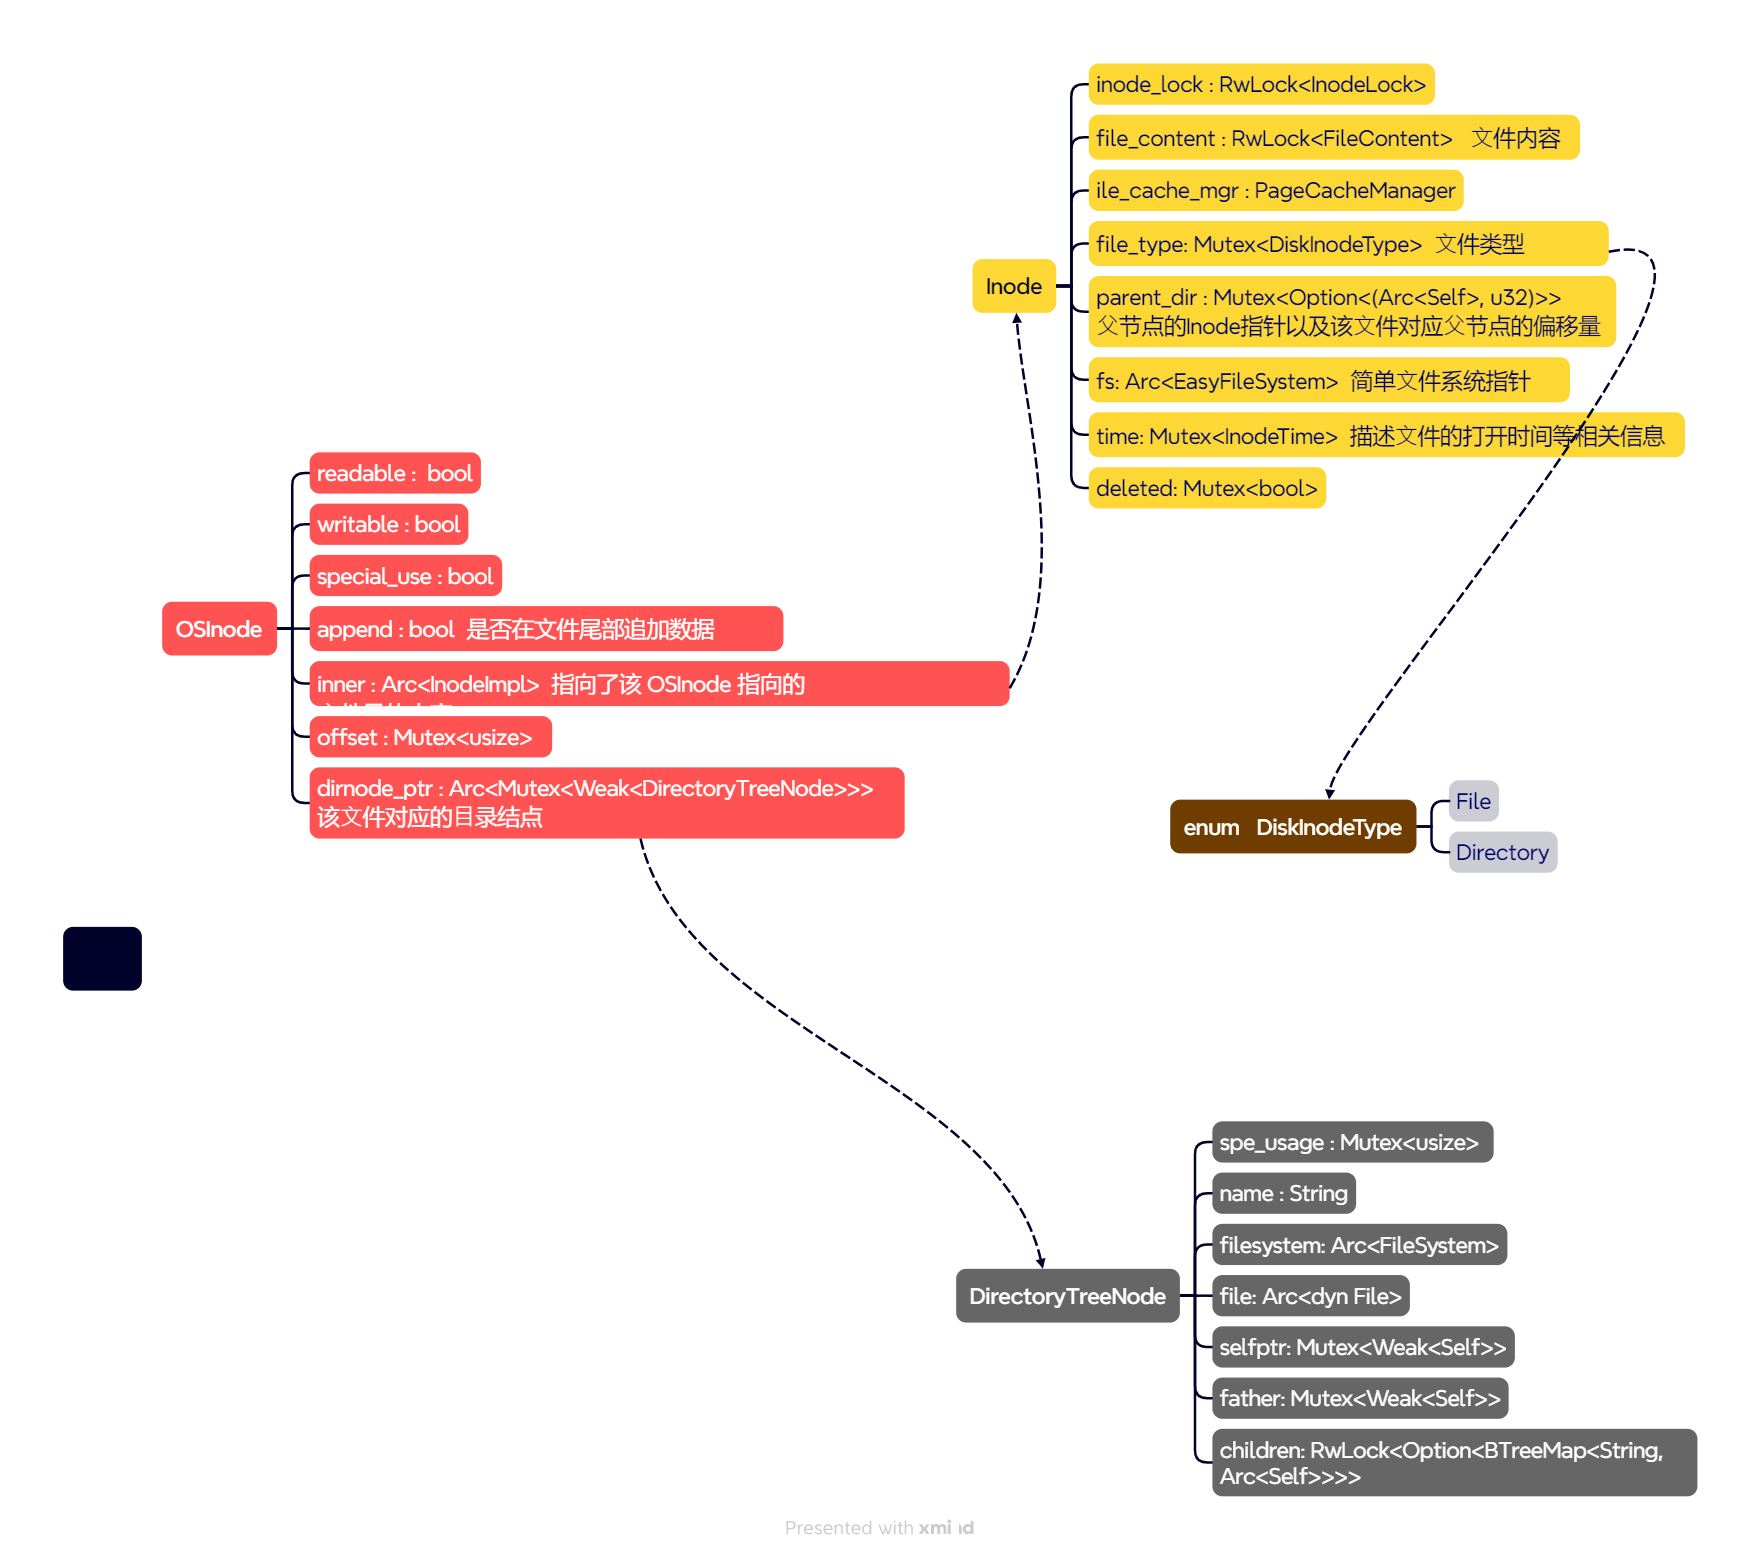
\includegraphics[width=14cm,height=11cm]{figures/07-05-NPUcore中数据结构之间的联系.png}
	\caption{NPUcore中数据结构之间的联系}
\end{figure} 

在NPUcore中,对于目录同样是以inode的形式存储在磁盘中,不
过为了更方便对文件进行各种操作,我们使用目录树结构来进行对
文件的定位。一方面我们可以使用 OSInode 来寻找其所在的目
录指针dirnode\_ptr,另一方面可以通过 directoryTreeNode 来找到其对
应的文件(夹) file 。

\begin{lstlisting}[language=Rust]
// os/src/fs/fat32/directory_tree.rs
pub struct DirectoryTreeNode {
	/// If this is a directory
	/// 1. cwd
	/// 2. mount point
	/// 3. root node
	/// If this is a file
	/// 1. executed by some processes
	/// This parameter will add 1 when
	opening
	///
	pub nlink_count : Mutex<u32>,
	在通过文件树寻找制定文件的过程中,首先会判断文件的路径前缀
	是否在路径缓存中,这样使大量文件操作效率更高,同时
	NPUcore也对一些默认的路径进行了路径的转化。
	文件描述符层
	spe_usage: Mutex<usize>,
	name: String,
	filesystem: Arc<FileSystem>,
	file: Arc<dyn File>,
	selfptr: Mutex<Weak<Self>>,
	father: Mutex<Weak<Self>>,
	children: RwLock<Option<BTreeMap<String,
	Arc<Self>>>>,
}
\end{lstlisting}

\begin{lstlisting}[language=Rust]
// src/os/fs/fat32/inode.rs
pub struct OSInode {
	//nlink_count : Mutex<usize>,
	readable: bool,
	writable: bool,
	special_use: bool,
	append: bool,
	inner: Arc<InodeImpl>,
	offset: Mutex<usize>,
	dirnode_ptr:
	Arc<Mutex<Weak<DirectoryTreeNode>>>,
}
\end{lstlisting}

内核全局维护了一个全局的目录节点向量 DIRECTORY\_VEC,记录当前系统所在的目录:
\begin{lstlisting}[language=Rust]
	static ref DIRECTORY_VEC: Mutex<
	(Vec<Weak<DirectoryTreeNode>>, usize)> = Mutex::new((Vec::new(), 0));
\end{lstlisting}

同时内核记录了根目录节点 ROOT,它的目录是空字符串:

\begin{lstlisting}[language=Rust]
	pub static ref ROOT: Arc<DirectoryTreeNode> = {
		let inode = DirectoryTreeNode::new(
		"".to_string(),
		Arc::new(FileSystem::new(FS::Fat32)),
		OSInode::new(InodeImpl::root_inode(&FILE_SYSTEM)),
		Weak::new()
		);
		inode.add_special_use();
		inode
	};
\end{lstlisting}

在通过文件树寻找制定文件的过程中,首先会判断文件的路径前缀
是否在路径缓存中,这样使大量文件操作效率更高,同时
NPUcore也对一些默认的路径进行了路径的转化。

